% !TeX root = RJwrapper.tex
\title{knitrdata: A Tool for Creating Standalone Rmarkdown Source Documents}
\author{by David M. Kaplan}

\maketitle

\abstract{%
Though Rmarkdown is a powerful tool for integrating text with code for analyses in a single source document exportable to a variety of output formats, until now there has been no simple way to integrate the data behind analyses into Rmarkdown source documents. The \texttt{knitrdata} package makes it possible for arbitrary text and binary data to be integrated directly into Rmarkdown source documents via implementation of a new \texttt{data} chunk type. The package includes command-line and graphical tools that facilitate creating and inserting \texttt{data} chunks into Rmarkdown documents, and the treatment of \texttt{data} chunks is highly configurable via chunk options. These tools allow one to easily create fully standalone Rmarkdown source documents integrating data, ancillary formatting files, analysis code and text in a single file. Used properly, the package can facilitate open distribution of source documents that demonstrate computational reproducibility of scientific results.
}

\hypertarget{introduction}{%
\section{Introduction}\label{introduction}}

The basic principles of open science are that the data, research methodologies and analysis tools (e.g., the specific computational tools) used for scientific research should be made publicly available so that others can confirm and validate scientific analyses. Open science is particularly important for studies and disciplines for which true experimental replication is often difficult or impossible due to spatial, temporal or individual specificity {[}e.g., we cannot replicate Earth; Powers and Hampton (2019){]}. In these cases, computational reproducibility, i.e., the ability to reproduce analytic results given the original data and analysis code, can still be achieved and can provide significant credibility to results (Powers and Hampton 2019). Though scientists, governments and journals often place great emphasis on access to raw data (Cassey and Blackburn 2006; Lowndes et al. 2017), it is important to remember that computational reproducibility can only be assured if data, methods, computational tools and the relationships between these are \emph{all} openly accessible. Even when data are made publicly available, there are often significant gaps between the Methods section of a publication and the raw data that complicate reproducibility without access to the detailed code used to generate results. It is, therefore, essential for computational reproducibility that the code used to generate results be distributed along with the data and the publication itself. Though there are a number of potential ways to distribute all these elements together, probably the most common current approach is to place the data in a publicly accessible data store (e.g., \href{https://datadryad.org}{Dryad}) and to associate the code with the publication via the supplementary material and/or by including it in the data store. Though this is a perfectly viable approach that can greatly enhance transparency of research, it physically separates data from analysis code and interpretation of results, potentially leading to confusion and/or loss of information regarding how these different element interrelate. At times, it would be more convenient, transparent and/or effective to join all the elements into a single document. The R package presented here, \CRANpkg{knitrdata} (Kaplan 2020a), provides tools for doing just that - integrating data directly into Rmarkdown source documents so that data, code for analyses and text interpreting results are all available in a single file.

Rmarkdown (Allaire, Xie, McPherson, et al. 2022) has become an increasingly popular tool for generating rich scientific documents while maintaining a source document that makes explicit the relationship between text and specific analyses used to produce results (Xie 2014; Lowndes et al. 2017). In a nutshell, Rmarkdown source documents are text documents comprised of two major elements: structured text that make up the headings and paragraphs of the document, and blocks of code (typically, but not exclusively, R code) for doing analyses and generating figures and tables. Rmarkdown source documents can be processed into a variety of final output formats, including PDF documents formatted for scientific publication. During this processing, the blocks of code in the source document are executed and used to augment the final output document with figures, tables and analytic results. In addition to providing a single source document that includes both written text and code for carrying out analyses, Rmarkdown has other benefits for open science, such as requiring the user to provide fully functioning code that runs from start to end without errors and facilitating reuse and updating of documents when new data arrives.

Until now, however, it has been difficult to integrate the raw data itself that are the bases for analyses directly into Rmarkdown source documents. Typically, data are placed in external files that are accessed via R code contained in the Rmarkdown source document that is executed during the knitting. As previously mentioned, this has the disadvantage of physically separating data from analysis code and text contained in the Rmarkdown source document, potentially leading to confusion and/or information loss. Furthermore, on a practical level, it often can be extremely convenient to merge all pertinent information into a single source document (e.g., to facilitate collaboration on an Rmarkdown source document). \texttt{knitrdata} provides a simple mechanism for integrating arbitrary text or binary data directly into Rmarkdown source documents, thereby allowing one to create standalone source documents that include all the elements necessary for conducting analyses. This integration is done with minimal additional formatting of the data (e.g., allowing one to insert comma-separated value (CSV) data without escaping quotation marks directly into Rmarkdown documents) and in a way that clearly visually separates data from R code, thereby facilitating comprehension of the different elements that contribute to analyses. \texttt{knitrdata} also facilitates encryption of data integrated into Rmarkdown source documents, thereby allowing one to merge data with analysis code and text even in cases where industrial or ethical privacy constraints restrict data access to a specific group of individuals.

Below, I briefly provide a conceptual overview of how \texttt{knitrdata} works, presenting some simple examples of its use and the tools available to facilitate integrating data into Rmarkdown source documents. I then discuss typical use cases and workflows for development of Rmarkdown source documents with \texttt{knitrdata}, as well as a number of potential caveats for its use. I conclude by reflecting on the value of \texttt{knitrdata} for achieving computational reproducibility and its place within the growing pantheon of tools that make Rmarkdown an increasingly essential tool for research.

\hypertarget{knitrdata-installation-and-usage}{%
\section{knitrdata installation and usage}\label{knitrdata-installation-and-usage}}

The \texttt{knitrdata} package is available on \href{https://cran.r-project.org/package=knitrdata}{CRAN}, though the latest version can be installed from \href{https://github.com/dmkaplan2000/knitrdata}{github} using the \CRANpkg{remotes} (Csárdi et al. 2021) package:

\begin{verbatim}
remotes::install_github("dmkaplan2000/knitrdata",
                        build_vignettes=TRUE)
\end{verbatim}

Once the package has been installed, all that is needed to use the functionality provided by the package in a Rmarkdown source document is to load the library at the start of the document, typically in the \texttt{setup} chunk:

\begin{verbatim}
library(knitrdata)
\end{verbatim}

\hypertarget{conceptual-overview-of-knitrdata}{%
\section{\texorpdfstring{Conceptual overview of \texttt{knitrdata}}{Conceptual overview of knitrdata}}\label{conceptual-overview-of-knitrdata}}

To understand how \texttt{knitrdata} works and the functionality it provides, one must first understand some of the terminology and functioning of Rmarkdown itself. As previously mentioned, Rmarkdown documents are a combination of text written in \emph{markdown}, a simple, structured text format that can be translated into a large number of final output formats, and code for doing analyses that can augment the final output document with analytic results, tables and figures. The code is contained in specially delimited blocks, referred to as \emph{chunks}. For example, adding the following to an Rmarkdown document:

\begin{verbatim}
```{r}
plot(-5:5,(-5:5)^2,type="l")
```
\end{verbatim}

would add a plot of a parabola to the final output document. The process of translating a Rmarkdown document into a final output document is known as \emph{knitting}, and this process is carried out using (often implicitly via RStudio) the \CRANpkg{knitr} package (Xie 2015).

Though code chunks typically contain R code, \texttt{knitr} supports a large number of other \emph{language engines}, allowing one to integrate analyses in a number of other computer languages, including C, Python and SQL. For example, one could use the SQL language engine to import the contents of a database table into the R environment by including the following chunk in a Rmarkdown source document:

\begin{verbatim}
```{sql connection="dbcon",output.var="d"}
SELECT * FROM "MyTable";
```
\end{verbatim}

During knitting, this will create in the R environment a variable \texttt{d} containing the contents of the table \texttt{MyTable} accessible via the (previously created) active R database connection \texttt{dbcon}. Note that the name of the database connection and the name of the output variable are supplied in the chunk header via what are known as \emph{chunk options}. Though this database table could be imported into the R environment without the SQL language engine using R code:

\begin{verbatim}
```{r}
d = dbGetQuery(dccon,"SELECT * FROM \"MyTable\";")
```
\end{verbatim}

the use of the SQL language engine has both practical and conceptual advantages. On the practical side, it avoids the need to escape quotation marks and allows text editors to recognize and highlight the code as SQL, both of which becoming increasingly valuable as the length and complexity of SQL queries increase. On the conceptual side, using the SQL engine visually separates database queries from R code and text, thereby better communicating the structure and functioning of analyses in Rmarkdown documents.

The \texttt{knitrdata} package works in many ways analogously to the SQL language engine, adding a new \texttt{data} language engine to the list of language engines known to \texttt{knitr} that is specifically designed to import raw ``data'' into the R environment and/or export it to external files. Here the term ``data'' is used in a very wide sense, including not only standard data tables (e.g., CSV text files) or binary data (e.g., RDS files, NetCDF files, images), but also text and formatted text (e.g., XML files, BibTeX files). For example, placing the following chunk in a Rmarkdown source document will, during the knitting process, create in the R environment a data frame \texttt{d} containing the contents of the comma-separated values (CSV) data in the chunk (provided that the \texttt{knitrdata} package has been previously loaded as described above):

\begin{verbatim}
```{data output.var="d",loader.function=read.csv}
name,score
David M. Kaplan,1.2
The man formerly known as "Prince",3.4
Peter O'Toole,5.6
```
\end{verbatim}

As with the SQL language engine, the name of the output variable for the chunk is supplied with a chunk option and in this example a \texttt{loader.function} option instructs \texttt{knitrdata} how to translate the contents of the chunk into a usable R object (in this example the R function \texttt{read.csv} is used to translate the CSV data into a data frame).

There are of course a number of other ways that such a simple data table could be imported into the R environment, including via an external data file or directly in R code, one approach to which might be:

\begin{verbatim}
```{r}
d = read.csv(textConnection(
"name,score
David M. Kaplan,1.2
The man formerly known as \"Prince\",3.4
Peter O'Toole,5.6
"))
```
\end{verbatim}

However, using the \texttt{data} language engine has much the same practical and conceptual advantages as the SQL data language engine, avoiding the need for escaping certain characters and visually separating data from code, both of which become increasingly valuable as dataset size increases.

Incorporating binary data into Rmarkdown source documents is a bit more complicated as the data must first be \emph{encoded} as ASCII text (see the Section below on \protect\hyperlink{binary}{Binary data chunks} for details), but the basic principles are the same - encoded binary data is incorporated into a \texttt{data} chunk and chunk options are used to tell \texttt{knitrdata} how to decode the data and load it into the R environment during knitting (see Table \ref{tab:knitrdatachunkops} for a full list of \texttt{data} chunk options). There is also the possibility of saving \texttt{data} chunk contents out to external files using the \texttt{output.file} chunk option. This option is particularly useful for integrating into Rmarkdown source documents ancillary text files used in the final formatting of the output of the knitting process, such as BibTeX files with references, LaTeX style files for PDF output and CSS style files for HTML output. For example, the following chunk would export a BibTeX reference to a file named \texttt{refs.bib}, taking care not to overwrite an existing file with the same name {[}though note that similar functionality can also be achieved with the \texttt{cat} language engine; Xie, Dervieux, and Riederer (2020){]}:

\begin{verbatim}
```{data output.file = "refs.bib", eval=!file.exists("refs.bib")}

@book{allaireRmarkdownDynamicDocuments2020,
  title = {Rmarkdown: {{Dynamic}} Documents for r},
  author = {Allaire, JJ and Xie, Yihui and McPherson, Jonathan and Luraschi, Javier and Ushey, Kevin and Atkins, Aron and Wickham, Hadley and Cheng, Joe and Chang, Winston and Iannone, Richard},
  year = {2020}
}
```
\end{verbatim}

As code chunks are processed during knitting before generating the final output document, these files can be generated at any point during the knitting process using \texttt{data} chunks (in particular, it is often most practical to place this information at the end of a Rmarkdown document).

\begin{longtable}[]{@{}
  >{\raggedright\arraybackslash}p{(\columnwidth - 2\tabcolsep) * \real{0.2740}}
  >{\raggedright\arraybackslash}p{(\columnwidth - 2\tabcolsep) * \real{0.7260}}@{}}
\caption{\label{tab:knitrdatachunkops} Full list of knitrdata chunk options.}\tabularnewline
\toprule
\begin{minipage}[b]{\linewidth}\raggedright
Chunk option
\end{minipage} & \begin{minipage}[b]{\linewidth}\raggedright
Description
\end{minipage} \\
\midrule
\endfirsthead
\toprule
\begin{minipage}[b]{\linewidth}\raggedright
Chunk option
\end{minipage} & \begin{minipage}[b]{\linewidth}\raggedright
Description
\end{minipage} \\
\midrule
\endhead
\texttt{decoding.ops} & A list with additional arguments for
\texttt{data\_decode}. Currently only useful for passing
the \texttt{verify} argument to
\CRANpkg{gpg}::\texttt{gpg\_decrypt} (Ooms 2022) for \texttt{gpg}
encrypted chunks. \\
\texttt{echo} & A boolean indicating whether or not to include
chunk contents in Rmarkdown output. Defaults to
\texttt{FALSE}. \\
\texttt{encoding} & One of \texttt{\textquotesingle{}asis\textquotesingle{}}, \texttt{\textquotesingle{}base64\textquotesingle{}} or \texttt{\textquotesingle{}gpg\textquotesingle{}}. Defaults
to \texttt{\textquotesingle{}asis\textquotesingle{}} for \texttt{format=\textquotesingle{}text\textquotesingle{}} and \texttt{\textquotesingle{}base64\textquotesingle{}} for
\texttt{format=\textquotesingle{}binary\textquotesingle{}}. \\
\texttt{eval} & A boolean indicating whether or not to process the
chunk. Defaults to \texttt{TRUE}. \\
\texttt{external.file} & A character string with the name of a file whose
text contents will be used as if they were the
contents of the data chunk. \\
\texttt{format} & One of \texttt{\textquotesingle{}text\textquotesingle{}} or \texttt{\textquotesingle{}binary\textquotesingle{}}. Defaults to
\texttt{\textquotesingle{}text\textquotesingle{}}. \\
\texttt{line.sep} & Only used when \texttt{encoding=\textquotesingle{}asis\textquotesingle{}}. In this cases,
specifies the character string that will be used
to join the lines of the data chunk before export
to an external file, further processing or
returning the data. Defaults to
\texttt{knitrdata::platform.newline()}. \\
\texttt{loader.function} & A function that will be passed (as the first
argument) the name of a file containing the
(potentially decoded) contents of the data chunk. \\
\texttt{loader.ops} & A list of additional arguments to be passed to
\texttt{loader.function}. \\
\texttt{max.echo} & An integer specifying the maximum number of lines
of data to echo in the final output document.
Defaults to 20. If the data exceeds this length,
only the first 20 lines will be shown and a final
line indicating the number of ommitted lines will
be added. \\
\texttt{md5sum} & A character string giving the correct md5sum of
the \emph{decoded} chunk data. If supplied, the md5sum
of the decoded data will be calculated and
compared to the supplied value, returning an error
if the two do not match. \\
\texttt{output.file} & A character string with the filename to which the
chunk output will be written. At least one of
\texttt{output.var} or \texttt{output.file} must always be
supplied. \\
\texttt{output.var} & A character string with the variable name to which
the chunk output will be assigned. At least one of
\texttt{output.var} or \texttt{output.file} must always be
supplied. \\
\bottomrule
\end{longtable}

Using \texttt{data} chunks, just about any data or information that would typically be stored in external files can be integrated directly into Rmarkdown source documents. In particular, this permits creating standalone Rmarkdown source documents that can be knitted without need for external data files, thereby uniting text, code and data in a single source document.

Note that this is different from the \texttt{self\_contained} YAML header option permitted by some Rmarkdown output formats, notably HTML output formats. This option attempts to create a single \emph{output} file that contains everything needed to visualize the final output document (e.g., in the case of HTML documents, the output HTML file will contain any CSS styles, javascript libraries and/or images used by the document), but it says nothing about whether or not external files are needed to knit the Rmarkdown source document (i.e., it is relevant to the output side of knitting, not the input side). In fact, a source document can be standalone in that all data and formatting files needed for knitting are incorporated within it using \texttt{data} chunks, but the final output (HTML) document may not be self contained because it relies on external files or libraries for visualization, and vice-versa (i.e., standalone source documents and standalone output documents are two separate and independent concerns).

Under the hood, the way \texttt{knitrdata} works is by adding (using the \texttt{knitr::knit\_engines\$set()} function) to the list of language engines that \texttt{knitr} maintains internally a \texttt{data} entry that points to a function inside the \texttt{knitrdata} package that processes \texttt{data} chunks (specifically the \texttt{eng\_data} function, though users would typically not interact directly with this function). When knitting a Rmarkdown document, \texttt{knitr} will call this function each time a \texttt{data} chunk is encountered, passing it both the textual contents of the chunk and any chunk options. The function then uses this information to process the chunk, decoding it if necessary (via the \texttt{format} and \texttt{encoding} chunk options) and returning it as either a variable in the R environment (\texttt{output.var} chunk option) and/or an external file (\texttt{output.file} chunk option) after any additional processing has been carried out (via, e.g., the \texttt{loader.function} chunk option).

\hypertarget{text-data-chunks}{%
\subsection{Text data chunks}\label{text-data-chunks}}

Though a basic example of a \texttt{data} chunk containing CSV tabular data has been presented in the previous section, it is useful to develop that example a bit more to better understand the functioning of \texttt{knitrdata}. The simplest \texttt{data} chunks contain plain text that is read, but not processed by \texttt{knitrdata}. For example, omitting the \texttt{loader.function} chunk option from the previously presented \texttt{data} chunk with CSV data produces a different outcome:

\begin{verbatim}
```{data output.var="txt"}
site,density
a,1.2
b,3.4
c,5.6
```
\end{verbatim}

During the knitting process, this will place the text contents of the chunk into a R variable named \texttt{txt}, but no further processing of the text will be carried out (i.e., the variable \texttt{txt} will contain the literal text contents of the chunk, excluding the header with the chunk options and the tail). One could later convert the text into a R \texttt{data.frame} using the \texttt{read.csv} command in a R chunk placed after the \texttt{data} chunk:

\begin{verbatim}
```{r}
d <- read.csv(text=txt)
```
\end{verbatim}

The \texttt{loader.function} chunk option used in the initial \texttt{data} chunk example above causes \texttt{knitrdata} to combine into one process the two steps of (1) reading in the chunk contents and (2) converting them into a usable R data object. Whereas the first of these steps, reading the chunk contents, is carried out for all \texttt{data} chunks, the second only occurs if the \texttt{loader.function} chunk option is given. \texttt{loader.function} should be a function that takes in the name of a file containing the chunk contents and returns the processed contents. Though \texttt{read.csv} is likely to be a common choice, there are many other possibilities including \texttt{readRDS}, \texttt{read.csv2}, \texttt{scan}, \texttt{png::readPNG} and custom, user-defined functions. One can also supply a list of additional input arguments to the loader function using the \texttt{loader.ops} chunk option (e.g., one could change the expected separator in CSV data using \texttt{loader.ops=list(sep="\textbar{}")}).

\hypertarget{binary}{%
\subsection{Binary data chunks}\label{binary}}

Though text data chunks can integrate into Rmarkdown source documents many small- to medium-sized tabular data sets, binary data formats, such as RDS files, are more convenient for more complicated and/or larger data sets. Incorporating binary data into Rmarkdown documents requires additional steps relative to text data: encoding the binary data as text and telling the \texttt{data} chunk how to decode the encoded data. \texttt{knitrdata} provides tools for simplifying these two steps that currently support encoding and decoding of two widely-used encodings: \texttt{base64} and \texttt{gpg}. \href{https://en.wikipedia.org/wiki/Base64}{\texttt{base64}} is a standard format for encoding binary data as ASCII text based on translation of 6 bits of information into one of 64 alphanumeric and symbolic ASCII characters. Base64 encoded data looks like a somewhat intimidating jumble of characters, but the format is extremely widely used behind the scenes in many common web applications, such as email attachments and embedding images in HTML pages. In particular, \texttt{base64} is widely supported by a number of software packages and programming languages, including R, Python, Matlab and Julia, so \texttt{base64} encoded data is highly readable and likely to remain so for a very long time.

\texttt{gpg}, standing for \href{https://gnupg.org/}{GNU Privacy Guard}, is a standard protocol for encrypting information so that only those with specific decryption keys can have access. This format can be used to ensure that only specific individuals can actually read and utilize the data contained in a Rmarkdown source document, as might be necessary when dealing with confidential (e.g., medical or trade-secret) data. Here, I focus primarily on \texttt{base64} encoding as this is the simplest and likely most common format for binary \texttt{data} chunks, and a full description of the configuration and use of GPG is beyond the scope of this document. The detailed use of \texttt{gpg} is, however, described in the package vignette.

Though \texttt{knitrdata} users rarely need to encode data by hand as the package provides \protect\hyperlink{addins}{graphical tools} for this, it is instructive to have a basic understanding of the underlying functions for encoding and decoding data: \texttt{data\_encode} and \texttt{data\_decode}. \texttt{data\_encode} takes the name of the file containing the data and the name of the encoding format, and it returns the encoded data that one would incorporate into a \texttt{data} chunk, either to the R command line or to a file. For example, if one saves the data frame \texttt{d} created in the previous section to a binary \texttt{RDS} file:

\begin{verbatim}
saveRDS(d,"data.RDS")
\end{verbatim}

then one can encode this data as \texttt{base64} using:

\begin{verbatim}
b64 = knitrdata::data_encode("data.RDS","base64")
cat(b64)
\end{verbatim}

\begin{verbatim}
#> H4sIAAAAAAAAA12OvQ+CMBDFKx+DGNTExPk2J1lc3HQwLsbIgInrBUokQmsKkbj5
#> PzsrXrEMekn72l/f693JY4zZzLEsZrt0ZO4x2s6XxCZ0sWiNvwbWJx1t8JYlsA9g
#> h9cchcEQnTkUKCCVquAqv8NFyFoAlhCqTMTc+PyQV1zBYRZJmXMCQ/336rloaz0w
#> Ok3bYjQVvfdM2BVY8NIMZBnoaNgZylgq/p+Kcyy7VAe9BCsMUqWzv/a+knXQNfJ1
#> owdtTdO8SN4fPb8RnS0BAAA=
\end{verbatim}

This jumble of characters starting with \texttt{"H4sI"} is the base64 encoded contents of the binary file that one would place in a \texttt{data} chunk. For large files, it is often more practical to output the encoded data to a file by supplying the \texttt{output} argument:

\begin{verbatim}
knitrdata::data_encode("data.RDS","base64",
                       output="data.RDS.base64")
\end{verbatim}

GPG encoding works similarly to base64 encoding, but one must change the format from \texttt{"base64"} to \texttt{"gpg"} and specify the encryption key (i.e., the receiver ID) to be used to encrypt the data.

Once one has the encoded data, one can use it in a \texttt{data} chunk by supplying the \texttt{format="binary"} chunk option and, optionally, an appropriate \texttt{loader.function} to convert the data into a R object:

\begin{verbatim}
```{data format="binary",output.var="d",loader.function=readRDS}
H4sIAAAAAAAAA12OvQvCMBDFz48OKn6A4Hybk11c3HQQFxE7VHA9aopimkgiFjf/
Z2etl5oOesO93I/3crdvA0ADmnXuAT8h2MWryYynIQ9MYfA1QIu1v6Tb6YCbENd0
kaQ8xvgoMCOFqTaZMPKOZ6VzhWQxMieVCO/rRuIqDG7HsdZSMOi5v+fPaVmLjtdR
WhaUV0HNhwNFmbD+oLqHTQcrg020Ef+pRJKtUhVsH+hKYWpc9tfeMjoPq0Vdt+jB
rSiKF8v7A6bdy9EtAQAA
```
\end{verbatim}

During knitting, this chunk will be processed, decoding the encoded binary RDS file and loading it into the variable \texttt{d} using the \texttt{readRDS} function. \texttt{knitrdata} will by default assume that the encoding is base64 when \texttt{format="binary"}, but one can also specify the chunk option \texttt{encoding="base64"} for increased clarity. For GPG encoded data, one would use \texttt{encoding="gpg"}. As with text \texttt{data} chunks, one can alternatively output the decoded contents of the chunk to a file (\texttt{output.file} option) or return it to the R session as a \texttt{raw} binary vector (by not supplying a \texttt{loader.function}).

\hypertarget{addins}{%
\subsection{RStudio add-ins for creating data chunks}\label{addins}}

\begin{figure}
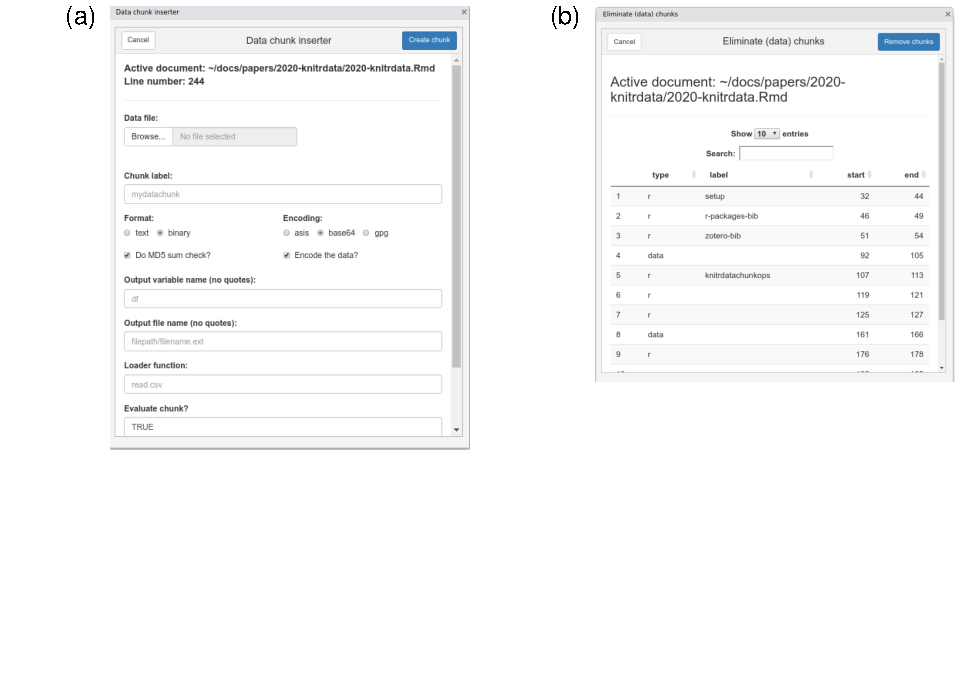
\includegraphics[width=400px]{2020-knitrdata_files/figure-latex/addinfigure-1} \caption{The (a) 'Insert filled data chunk' and (b) 'Remove chunks' RStudio add-ins included with knitrdata. The dialogues will open when selected from the 'Addins' menu of RStudio. They allow one to (a) insert a data chunk containing the contents of an existing external data file into an open Rmarkdown document, and (b) delete one or more chunks from an open Rmarkdown document.}\label{fig:addinfigure}
\end{figure}

As manually encoding data and creating \texttt{data} chunks can be complicated, particularly for large data files, \texttt{knitrdata} includes graphical RStudio add-ins that do all the hard work of incorporating data in Rmarkdown documents. The principal add-in is called \texttt{Insert\ filled\ data\ chunk} (Fig. \ref{fig:addinfigure}a). Though its use is meant to be largely self-explanatory, an instructional video is available on YouTube (Kaplan 2020b). The basic idea is that one opens a Rmarkdown source document in the RStudio editor, places the cursor at the location one wants to insert a \texttt{data} chunk and then activates the add-in. The add-in prompts for the name of the data file to be incorporated, as well as values for various \texttt{data} chunk output and processing options. Based on the type of data file selected, the add-in will attempt to select or suggest various appropriate options. For example, if a RDS file is chosen, then format will be set to \texttt{binary}, encoding will be set to \texttt{base64} and the loader function will be set to \texttt{readRDS}. These defaults can be manually modified if not appropriate. The add-in also greatly facilitates and encourages the use of \protect\hyperlink{integrity}{MD5 sum data integrity checks}. After all options have been set, one clicks on \texttt{Create\ chunk} and an appropriately-formatted \texttt{data} chunk will be inserted in the active Rmarkdown source document at the cursor location.

\texttt{knitrdata} also provides a \texttt{Remove\ chunks} add-in that allows ones one to quickly delete unwanted (\texttt{data} and non-\texttt{data}) chunks (Fig. \ref{fig:addinfigure}b), as well as a set of functions for command-line examination, creation and removal of chunks from Rmarkdown documents (e.g., \texttt{create\_chunk}, \texttt{insert\_chunk}, \texttt{list\_rmd\_chunks}, \texttt{remove\_chunks}).

If one is not using RStudio to edit and knit Rmarkdown documents, then one can invoke the Skiny dialog to create \texttt{data} chunks directly from the command line using the \texttt{create\_data\_chunk\_dialog} function contained in the \texttt{knitrdata} package. In this case, chunk contents will be (silently) returned on the command line for later insertion in a Rmarkdown document.

\hypertarget{use-cases}{%
\section{Use cases}\label{use-cases}}

There are a number of use cases for the functionality provided by \texttt{knitrdata}, primary among them providing a single source for public diffusion of all information related to a publication or report, and/or making collaboration on Rmarkdown source documents simpler by eliminating or reducing the need for external files. A simple example of the prior is the Rmarkdown source document used to generate \href{https://github.com/dmkaplan2000/knitrdata_examples/blob/e5f59b7475a542bef41c60e8ee6652f656c9e377/2020-knitrdata.Rmd}{this publication}, which includes text \texttt{data} chunks for the tabular data in Table \ref{tab:knitrdatachunkops}, as well as the ancillary formatting files associated with the document (BibTeX and LaTeX style files), and encoded binary \texttt{data} chunks for the PNG images in Figs. \ref{fig:addinfigure} \& \ref{fig:openclosechunkfig}.

A more complicated example is the Rmarkdown source document for Wain et al. (2021), \href{https://github.com/dmkaplan2000/knitrdata_examples/blob/e5f59b7475a542bef41c60e8ee6652f656c9e377/wain.et.al.2020.standalone.Rmd}{publicly available on github}. In this case, we wished to provide a permanent public record of the methods used in the paper and ensure that results could be verified, while at the same time respecting confidentiality agreements with respect to fine scale fishing activity data used in the paper. To achieve this we integrated the fine scale data in the Rmarkdown source document as an encrypted GPG \texttt{data} chunk. This approach may have value for a wide number of other studies using sensitive economic, social or medical data. To provide a complete record of the paper in a single document, we also integrated the Rmarkdown source document for the online supplementary materials into a \texttt{data} chunk within the Rmarkdown source document for the paper itself. As this supplementary materials document contains Rmarkdown chunks that would otherwise confuse the knitting process if integrated as raw text inside a \texttt{data} chunk, we base64 encoded this source document before including it in a \texttt{data} chunk. The document also contains \texttt{data} chunks for small data tables and for exporting to external files the ancillary formatting files required for knitting the document (BibTeX references, the LaTeX style file, the CSL citation style file, etc.). Finally, during the knitting process, the document also generates a lightweight version of itself that does not include the main data chunk, using the functionality of the \texttt{knitrdata} package to remove large data chunks. Overall, \texttt{knitrdata} provided a convenient way of generating a single document that contained all the necessary information for generating the final publication, thereby demonstrating computational reproducibility for the publication.

The uses of \texttt{data} chunks tend to fall into one of four general, not mutually-exclusive use cases:

\begin{enumerate}
\def\labelenumi{\arabic{enumi})}
\tightlist
\item
  Integration of ancillary formatting files into the Rmarkdown source document, thereby reducing the number of external files needed to knit a document
\item
  Inclusion of small- to medium-sized tabular data used in analyses and/or for tables
\item
  Inclusion of larger data sets using encoded binary data
\item
  Inclusion of confidential data using GPG-encrypted \texttt{data} chunks
\end{enumerate}

Though the first of these use cases, integration of ancillary formatting files, can also be achieved with the \texttt{cat} language engine that is included with the \texttt{knitr} package (Xie, Dervieux, and Riederer 2020), \texttt{knitrdata} provides functionality that make this task easier and more secure. First, \texttt{knitrdata} allows for integrity checks on chunk contents that can control for unintentional modification of chunk contents (see the section on \protect\hyperlink{integrity}{data integrity} below). Second, RStudio add-ins provided by the \texttt{knitrdata} package facilitate the integration of data into Rmarkdown source documents and the use of integrity checks. Finally, encoding of text documents permits integrating files that contain Rmarkdown chunks or other formatting that would otherwise be problematic within a \texttt{cat} chunk.

The second of these use cases, tabular data, can also in principle be achieved using other tools in R, such as a \texttt{textConnection} as shown above or via functionality in the \CRANpkg{tibble} package (Müller and Wickham 2022). Nevertheless, the use of \texttt{data} chunks is generally more ergonomic and flexible for anything but the smallest data tables as it allows the user to format data exactly as it would be in an external CSV file, without additional markup or the need to escape quotation marks. As an example, the information contained in Table \ref{tab:knitrdatachunkops} was implemented in the source document for this paper as a \texttt{data} chunk as it contains lots of quotations and formatting that would have been tedious to include using other approaches.

The third and fourth use cases for \texttt{data} chunks, involving encoded binary data, are unique to \texttt{knitrdata} and allow for integration of complex data sets that would otherwise be very difficult to include in a Rmarkdown source document.

\hypertarget{workflow}{%
\section{Workflow}\label{workflow}}

When and in what ways to use the functionality provided by \texttt{knitrdata} during the development of a Rmarkdown source document requires some thought and depends to some degree on the project goals. If the goal is to create a final Rmarkdown source document that demonstrates computational reproducibility of a set of results, then it may not be necessary or practical to use \texttt{data} chunks during the development stages of the project as the use of \texttt{data} chunks necessarily weighs down a Rmarkdown source document with information (e.g., binary data) that may not be immediately useful to authors during development. In this case, it may be best to work initially as one has always done, relying on external files for data and formatting. External data and formatting files can be incorporated in \texttt{data} chunks at the end of development when it is time to generate a final archival/public version of a Rmarkdown source document.

On the other hand, if the objective of using \texttt{knitrdata} also includes reducing the complexity of collaborating on a Rmarkdown source document by reducing the number of external files necessary for knitting a document, then certain types of \texttt{data} chunks can be incorporated in a Rmarkdown source document during the initial phases of development with little impact on authors. Small- to medium-sized tabular data sets can be incorporated and this can have the benefit of making the tabular data visually available during the development process. Similarly, most ancillary formatting files can be placed at the very end of the Rmarkdown source document as these are only used after all chunks have been processed and, therefore, will not encumber the development process. Larger data sets, and in particular binary data sets, are a bit more problematic as they necessarily appear in the Rmarkdown source document before the data is used for analyses and will introduce significant amounts of text that are not human readable into the Rmarkdown source document. For this reason it may be best to leave incorporation of these data until the final stages of development, though see the sections below on \protect\hyperlink{filesize}{file size} and \protect\hyperlink{readable}{readability} for workarounds to these issues.

This latter workflow involving incorporation of \texttt{data} chunks in two distinct stages of development is what was used when creating the source document for Wain et al. (2021). Small data tables and formatting files were incorporated directly into the document from the start, but the larger data set that was the basis for statistical analyses and the Rmarkdown source document for the supplementary materials were only incorporated at the end of development to provide an archival source document for the paper capable of demonstrating computational reproducibility.

\hypertarget{caveats-and-concerns}{%
\section{Caveats and concerns}\label{caveats-and-concerns}}

There are a number caveats and concerns with respect to the use of \texttt{knitrdata}, all of which have some validity, but for which a number of simple approaches exist to limit their impact. Below, I discuss four of them: \protect\hyperlink{filesize}{file size}, \protect\hyperlink{readable}{document readability}, \protect\hyperlink{integrity}{data integrity} and \protect\hyperlink{security}{security}.

\hypertarget{filesize}{%
\subsection{Won't this create huge Rmarkdown files?}\label{filesize}}

Incorporation of large data sets into \texttt{data} chunks will significantly increase the file size of Rmarkdown source documents, potentially making them more difficult to work with. Though it is unlikely to be practical to place extremely large data sets in Rmarkdown source documents, there are many contexts where data sets are sufficiently small so as to be included directly in a Rmarkdown source document. For example, the 8 years of fine scale fishing data used in Wain et al. (2021) added about 2 MB to the size of the Rmarkdown document when incorporated as a (compressed) RDS file, a size that is manageable and well within the limits of typical email attachments. RStudio currently will not open Rmarkdown documents larger than 5 MB in size, effectively limiting the amount of data that can be placed in a document unless one is willing to forgo graphical editing tools (larger documents can be rendered from the command line using the \texttt{rmarkdown::render} function, but not the more convenient and common ``Knit'' button of RStudio). Despite being in the era of big data, many scientific studies use primary data sets that are smaller than this size limit. As for Wain et al. (2021), many experimental or field studies may rely on data sets that are relatively small, and building a standalone Rmarkdown source document for these studies is an effective approach to documenting all quantitative information needed to reproduce results.

\hypertarget{readable}{%
\subsection{Won't Rmarkdown source documents become unreadable?}\label{readable}}

\begin{figure}
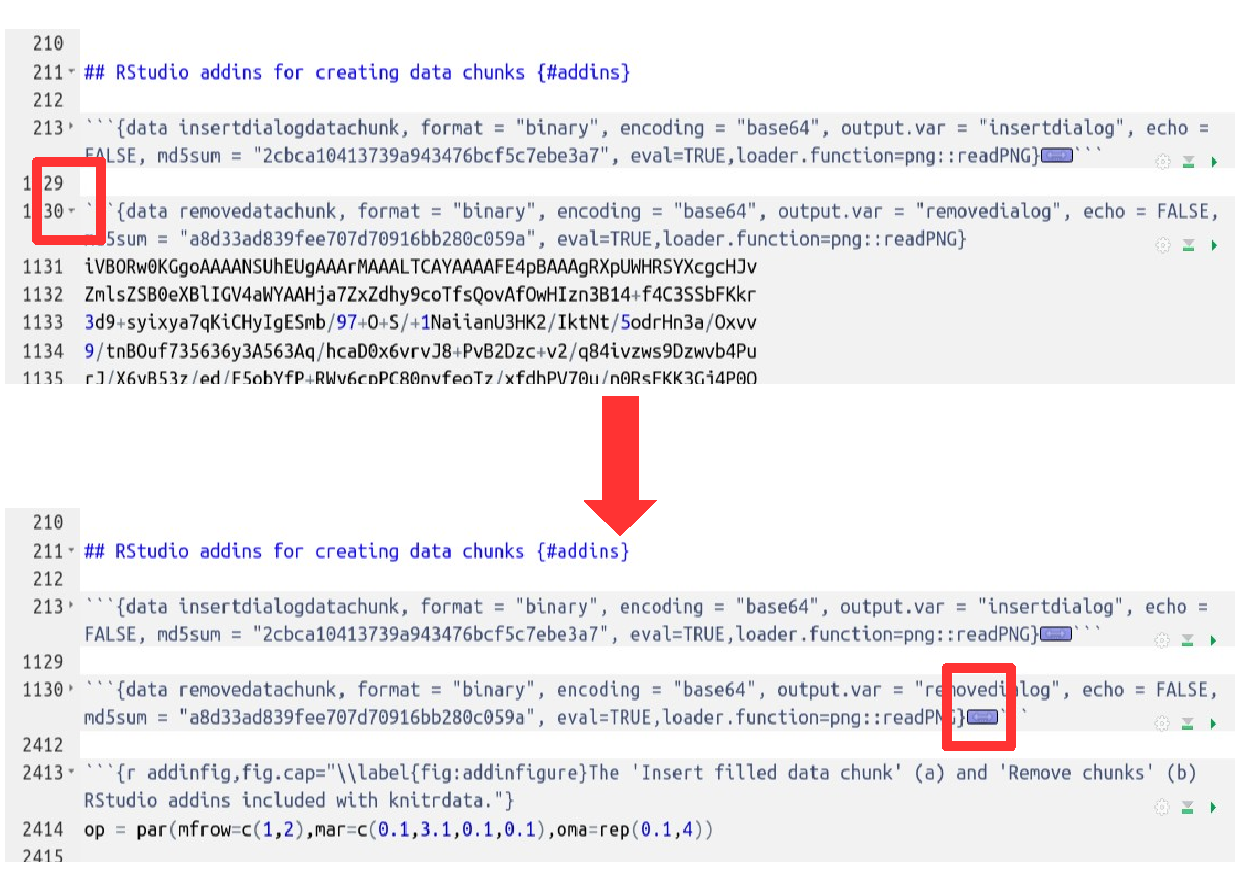
\includegraphics[width=400px]{open-close-chunk-fig} \caption{Images demonstrating before (top) and after (bottom) a data chunk has been hidden from view in the RStudio editor. The top image shows two base64-encoded data chunks, one of which is hidden, whereas the other is visible. In the bottom image, both chunks have been hidden. The control for hiding chunk contents (top) and an indicator of a hidden chunk (bottom) are highlighted with red boxes.}\label{fig:openclosechunkfig}
\end{figure}

Large amounts of encoded binary data are undoubtedly not pretty to look at, but readability is not necessarily the primary benefit of using Rmarkdown. Rather, completeness and the articulation of text and analyses are the strengths of Rmarkdown, benefits that \texttt{data} chunks enhance as opposed to diminish. Many Rmarkdown documents are already a complex mix of text and code that is difficult to read and manage without the tools RStudio and other editors provide to navigate the document, such as the ability to jump between sections and chunks. \texttt{data} chunks are no different in this sense, and use of informative chunk labels can greatly facilitate document navigation. Furthermore, RStudio includes the possibility of hiding chunk contents with a single click (Fig. \ref{fig:openclosechunkfig}), which can be quite practical when dealing with large \texttt{data} chunks. Once hidden, \texttt{data} chunk contents can be ignored, allowing one to edit the document unhindered.

\hypertarget{integrity}{%
\subsection{Won't a misplaced keystroke mess up my data?}\label{integrity}}

It is possible to unintentionally corrupt a \texttt{data} chunk due to a misplaced keystroke, particularly if the data is encoded and not readily human readable. However, the use of navigation tools and hiding of \texttt{data} chunk contents as described \protect\hyperlink{readable}{above} (Fig. \ref{fig:openclosechunkfig}) can drastically reduce interaction with chunk contents, thereby limiting the possibility for error. Furthermore, there are a number of methods to validate chunk contents, the simplest of which is to do a MD5 sum check using functionality included in \texttt{knitrdata}. A MD5 sum is a very large number (typically encoded in hexadecimal) derived from a file's contents that has a vanishingly small probability of being equal to that of another file if the files are not identical. \texttt{data} chunks can include a \texttt{md5sum} chunk option that specifies a MD5 sum that will be checked against that of the decoded chunk contents, generating an error if the two do not match. In this way, data corruption can be swiftly identified and corrected. The \texttt{Insert\ filled\ data\ chunk} RStudio add-in will by default calculate and include a MD5 sum check when inserting binary \texttt{data} chunks (and such a check can be optionally requested for text \texttt{data} chunks) so that users can easily benefit from these checks without having to worry about the details.

\hypertarget{are-there-security-concerns-when-using-knitrdata}{%
\subsection{\texorpdfstring{Are there security concerns when using \texttt{knitrdata}?}{Are there security concerns when using knitrdata?}}\label{are-there-security-concerns-when-using-knitrdata}}

Any time one runs code from a third party, there are security risks. Typically, code can write files to disk, potentially modifying essential files or installing malicious software. Rmarkdown source documents using the functionality of \texttt{knitrdata} are no different in this sense, though the practical risks may be more important as \texttt{knitrdata} may encourage users to knit entire documents to gain access to raw data and arbitrary data may be encoded in formats that are not human readable. Reducing these risks involves responsibilities for both the authors and the users of Rmarkdown source documents. For authors, the primary responsibilities are to assure that source documents cannot be modified by third parties between the author and the user, and to use best practices when carrying out file input and output during the knitting process. Integrity of source documents can be protected by using reputable websites with established security protocols for publishing Rmarkdown source documents, including, but not limited to, \href{https://github.com/}{github}, \href{https://zenodo.org/}{Zenodo} and the \href{https://datadryad.org}{Dryad}. Authors can also publish MD5 sums for Rmarkdown source documents so users can verify the integrity of those documents, though the security of those MD5 sums is only as strong as the websites on which MD5 sums and Rmarkdown source documents are published. Best practices for file input and output include using temporary files and/or relative paths entirely within the base directory containing the Rmarkdown source document when writing files to disk, using file names that are unique (e.g., avoiding generic names like \texttt{data.csv}) and performing checks for the existence of files with the same name before writing information to disk. The \texttt{Insert\ filled\ data\ chunk} RStudio add-in provided by \texttt{knitrdata} encourages the use of file existence checks in the \texttt{eval} chunk option controlling whether or not to process \texttt{data} chunks that write data to disk using the \texttt{output.file} chunk option, thereby avoiding overwriting existing files.

For users of Rmarkdown source documents, there are a number of simple steps one can take to avoid the most severe security risks. Knitting Rmarkdown source documents from an unprivileged user account and placing Rmarkdown source documents in new, empty directories can reduce the risks of the most malicious attacks. Users should also familiarize themselves with the workings of Rmarkdown source documents before knitting them and check for potentially problematic actions, such as use of absolute file paths and/or communication with external internet resources. This includes examination of the chunk options associated with \texttt{data} chunks (in particular, the \texttt{output.file} and \texttt{loader.function}). If one is primarily interested in just the raw data contained in \texttt{data} chunks within a Rmarkdown source document, then RStudio permits manual execution of individual chunks. This includes execution of \texttt{data} chunks, which can be processed individually using the \texttt{Run\ current\ chunk} button of RStudio once the \texttt{knitrdata} library has been loaded.

\hypertarget{conclusion}{%
\section{Conclusion}\label{conclusion}}

\texttt{knitrdata} provides a simple, but effective, tool for integrating arbitrary data into Rmarkdown source documents. If used appropriately, this can help assure computational reproducibility of many scientific documents by allowing one to integrate all relevant external files and data directly into a single Rmarkdown source document. Anyone who has attempted to validate the results in a publication by requesting the associated data has potentially encountered, if they managed to get the data, a set of one or more data tables with limited metadata and only the publication itself as documentation of the methods. Validating publication results under these conditions is often difficult and time consuming. By encouraging the integration of data, code for carrying out analyses, and text interpreting results in standalone Rmarkdown source documents, Rmarkdown with \texttt{knitrdata} can make it much easier to understand, reproduce and validate the details of scientific analyses. This combination can be particularly powerful when combined with other enhancements to Rmarkdown that make it possible to produce a wide variety of sophisticated scientific documents entirely within the confines of Rmarkdown, such as \CRANpkg{bookdown} (Xie 2022), \CRANpkg{rticles} (Allaire, Xie, Dervieux, et al. 2022) and \CRANpkg{starticles} (Kaplan 2022) for producing books and scientific publications with Rmarkdown, \CRANpkg{citr} (Aust 2019) for bibliographic citations, and \CRANpkg{kableExtra} (Zhu 2021) for producing sophisticated data tables.

\hypertarget{online-supporting-information}{%
\section{Online supporting information}\label{online-supporting-information}}

The Rmarkdown source documents for this publication and Wain et al. (2021) are available online at \url{https://github.com/dmkaplan2000/knitrdata_examples}. Additional examples and the package vignette are available in the \texttt{knitrdata} package itself.

\hypertarget{acknowledgements}{%
\section{Acknowledgements}\label{acknowledgements}}

I would like to thank my colleagues at the MARBEC laboratory in Sète, France for numerous conversations that encouraged me to develop the \texttt{knitrdata} package. I would also like to thank Yihui Xie for advice and encouragement regarding the development of the package. The handling editor and an anonymous reviewer provided valuable feedback that significantly improved the manuscript.

\hypertarget{references}{%
\section*{References}\label{references}}
\addcontentsline{toc}{section}{References}

\hypertarget{refs}{}
\begin{CSLReferences}{1}{0}
\leavevmode\vadjust pre{\hypertarget{ref-R-rticles}{}}%
Allaire, JJ, Yihui Xie, Christophe Dervieux, R Foundation, Hadley Wickham, Journal of Statistical Software, Ramnath Vaidyanathan, et al. 2022. \emph{Rticles: Article Formats for r Markdown}. \url{https://github.com/rstudio/rticles}.

\leavevmode\vadjust pre{\hypertarget{ref-R-rmarkdown}{}}%
Allaire, JJ, Yihui Xie, Jonathan McPherson, Javier Luraschi, Kevin Ushey, Aron Atkins, Hadley Wickham, Joe Cheng, Winston Chang, and Richard Iannone. 2022. \emph{Rmarkdown: Dynamic Documents for r}. \url{https://CRAN.R-project.org/package=rmarkdown}.

\leavevmode\vadjust pre{\hypertarget{ref-R-citr}{}}%
Aust, Frederik. 2019. \emph{Citr: RStudio Add-in to Insert Markdown Citations}. \url{https://github.com/crsh/citr}.

\leavevmode\vadjust pre{\hypertarget{ref-casseyReproducibilityRepeatabilityEcology2006}{}}%
Cassey, Phillip, and Tim M. Blackburn. 2006. {``Reproducibility and {Repeatability} in {Ecology}.''} \emph{BioScience} 56 (12): 958--59. \url{https://doi.org/10.1641/0006-3568(2006)56\%5B958:RARIE\%5D2.0.CO;2}.

\leavevmode\vadjust pre{\hypertarget{ref-R-remotes}{}}%
Csárdi, Gábor, Jim Hester, Hadley Wickham, Winston Chang, Martin Morgan, and Dan Tenenbaum. 2021. \emph{Remotes: R Package Installation from Remote Repositories, Including GitHub}. \url{https://CRAN.R-project.org/package=remotes}.

\leavevmode\vadjust pre{\hypertarget{ref-R-knitrdata}{}}%
Kaplan, David M. 2020a. \emph{Knitrdata: Data Language Engine for Knitr / Rmarkdown}. \url{https://github.com/dmkaplan2000/knitrdata}.

\leavevmode\vadjust pre{\hypertarget{ref-kaplanUsingKnitrdataCreate2020}{}}%
---------. 2020b. {``Using Knitrdata to Create Standalone {Rmarkdown} Documents in {Rstudio}.''} https://www.youtube.com/watch?v=xX4YRAXYFxE.

\leavevmode\vadjust pre{\hypertarget{ref-R-starticles}{}}%
---------. 2022. \emph{Starticles: A Generic, Publisher-Independent Template for Writing Scientific Documents in Rmarkdown}. \url{https://github.com/dmkaplan2000/starticles}.

\leavevmode\vadjust pre{\hypertarget{ref-lowndesOurpathbetter2017}{}}%
Lowndes, Julia S. Stewart, Benjamin D. Best, Courtney Scarborough, Jamie C. Afflerbach, Melanie R. Frazier, Casey C. O'Hara, Ning Jiang, and Benjamin S. Halpern. 2017. {``Our Path to Better Science in Less Time Using Open Data Science Tools.''} \emph{Nature Ecology \& Evolution} 1 (6): 1--7. \url{https://doi.org/10.1038/s41559-017-0160}.

\leavevmode\vadjust pre{\hypertarget{ref-R-tibble}{}}%
Müller, Kirill, and Hadley Wickham. 2022. \emph{Tibble: Simple Data Frames}. \url{https://CRAN.R-project.org/package=tibble}.

\leavevmode\vadjust pre{\hypertarget{ref-R-gpg}{}}%
Ooms, Jeroen. 2022. \emph{Gpg: GNU Privacy Guard for r}. \url{https://github.com/jeroen/gpg}.

\leavevmode\vadjust pre{\hypertarget{ref-powersOpenScienceReproducibility2019}{}}%
Powers, Stephen M., and Stephanie E. Hampton. 2019. {``Open Science, Reproducibility, and Transparency in Ecology.''} \emph{Ecological Applications} 29 (1): e01822. \url{https://doi.org/10.1002/eap.1822}.

\leavevmode\vadjust pre{\hypertarget{ref-wainQuantifyingIncreaseFishing2021}{}}%
Wain, Gwenaëlle, Loreleï Guéry, David Michael Kaplan, and Daniel Gaertner. 2021. {``Quantifying the Increase in Fishing Efficiency Due to the Use of Drifting {FADs} Equipped with Echosounders in Tropical Tuna Purse Seine Fisheries.''} \emph{ICES Journal of Marine Science} 78 (1): 235--45. \url{https://doi.org/10.1093/icesjms/fsaa216}.

\leavevmode\vadjust pre{\hypertarget{ref-knitr2014}{}}%
Xie, Yihui. 2014. {``Knitr: A Comprehensive Tool for Reproducible Research in {R}.''} In \emph{Implementing Reproducible Computational Research}, edited by Victoria Stodden, Friedrich Leisch, and Roger D. Peng. Chapman; Hall/CRC. \url{http://www.crcpress.com/product/isbn/9781466561595}.

\leavevmode\vadjust pre{\hypertarget{ref-knitr2015}{}}%
---------. 2015. \emph{Dynamic Documents with {R} and Knitr}. 2nd ed. Boca Raton, Florida: Chapman; Hall/CRC. \url{https://yihui.org/knitr/}.

\leavevmode\vadjust pre{\hypertarget{ref-R-bookdown}{}}%
---------. 2022. \emph{Bookdown: Authoring Books and Technical Documents with r Markdown}. \url{https://CRAN.R-project.org/package=bookdown}.

\leavevmode\vadjust pre{\hypertarget{ref-XieMarkdownCookbook2020}{}}%
Xie, Yihui, Christophe Dervieux, and Emily Riederer. 2020. \emph{R {Markdown Cookbook}}. 1st edition. The {R Series}. {Boca Raton, Florida}: {CRC Press}.

\leavevmode\vadjust pre{\hypertarget{ref-R-kableExtra}{}}%
Zhu, Hao. 2021. \emph{kableExtra: Construct Complex Table with Kable and Pipe Syntax}. \url{https://CRAN.R-project.org/package=kableExtra}.

\end{CSLReferences}

\bibliography{2020-knitrdata.bib}

\address{%
David M. Kaplan\\
MARBEC\\%
Univ Montepllier, CNRS, Ifremer, IRD\\ Sète, France\\
Institute de Recherche pour le Developpement (IRD)\\%
UMR MARBEC\\ av. Jean Monnet\\ CS 30171\\ 34203 Sète cedex, France\\
%
\url{https://www.davidmkaplan.fr}\\%
\textit{ORCiD: \href{https://orcid.org/0000-0001-6087-359X}{0000-0001-6087-359X}}\\%
\href{mailto:david.kaplan@ird.fr}{\nolinkurl{david.kaplan@ird.fr}}%
}
